% Options for packages loaded elsewhere
\PassOptionsToPackage{unicode}{hyperref}
\PassOptionsToPackage{hyphens}{url}
%
\documentclass[
]{book}
\usepackage{amsmath,amssymb}
\usepackage{lmodern}
\usepackage{iftex}
\ifPDFTeX
  \usepackage[T1]{fontenc}
  \usepackage[utf8]{inputenc}
  \usepackage{textcomp} % provide euro and other symbols
\else % if luatex or xetex
  \usepackage{unicode-math}
  \defaultfontfeatures{Scale=MatchLowercase}
  \defaultfontfeatures[\rmfamily]{Ligatures=TeX,Scale=1}
\fi
% Use upquote if available, for straight quotes in verbatim environments
\IfFileExists{upquote.sty}{\usepackage{upquote}}{}
\IfFileExists{microtype.sty}{% use microtype if available
  \usepackage[]{microtype}
  \UseMicrotypeSet[protrusion]{basicmath} % disable protrusion for tt fonts
}{}
\makeatletter
\@ifundefined{KOMAClassName}{% if non-KOMA class
  \IfFileExists{parskip.sty}{%
    \usepackage{parskip}
  }{% else
    \setlength{\parindent}{0pt}
    \setlength{\parskip}{6pt plus 2pt minus 1pt}}
}{% if KOMA class
  \KOMAoptions{parskip=half}}
\makeatother
\usepackage{xcolor}
\IfFileExists{xurl.sty}{\usepackage{xurl}}{} % add URL line breaks if available
\IfFileExists{bookmark.sty}{\usepackage{bookmark}}{\usepackage{hyperref}}
\hypersetup{
  pdftitle={Leadership 663},
  pdfauthor={Mark Halvorson, Colin Madland, Scott Macklin},
  hidelinks,
  pdfcreator={LaTeX via pandoc}}
\urlstyle{same} % disable monospaced font for URLs
\usepackage{longtable,booktabs,array}
\usepackage{calc} % for calculating minipage widths
% Correct order of tables after \paragraph or \subparagraph
\usepackage{etoolbox}
\makeatletter
\patchcmd\longtable{\par}{\if@noskipsec\mbox{}\fi\par}{}{}
\makeatother
% Allow footnotes in longtable head/foot
\IfFileExists{footnotehyper.sty}{\usepackage{footnotehyper}}{\usepackage{footnote}}
\makesavenoteenv{longtable}
\usepackage{graphicx}
\makeatletter
\def\maxwidth{\ifdim\Gin@nat@width>\linewidth\linewidth\else\Gin@nat@width\fi}
\def\maxheight{\ifdim\Gin@nat@height>\textheight\textheight\else\Gin@nat@height\fi}
\makeatother
% Scale images if necessary, so that they will not overflow the page
% margins by default, and it is still possible to overwrite the defaults
% using explicit options in \includegraphics[width, height, ...]{}
\setkeys{Gin}{width=\maxwidth,height=\maxheight,keepaspectratio}
% Set default figure placement to htbp
\makeatletter
\def\fps@figure{htbp}
\makeatother
\setlength{\emergencystretch}{3em} % prevent overfull lines
\providecommand{\tightlist}{%
  \setlength{\itemsep}{0pt}\setlength{\parskip}{0pt}}
\setcounter{secnumdepth}{5}
\usepackage{booktabs}
\usepackage{amsthm}
\makeatletter
\def\thm@space@setup{%
  \thm@preskip=8pt plus 2pt minus 4pt
  \thm@postskip=\thm@preskip
}
\makeatother
\ifLuaTeX
  \usepackage{selnolig}  % disable illegal ligatures
\fi
\usepackage[]{natbib}
\bibliographystyle{apalike}

\title{Leadership 663}
\author{Mark Halvorson, Colin Madland, Scott Macklin}
\date{2022-03-22}

\begin{document}
\maketitle

{
\setcounter{tocdepth}{1}
\tableofcontents
}
\hypertarget{leadership-663}{%
\chapter{Leadership 663}\label{leadership-663}}

Examines the theoretical foundations and professional practices of coaching learners in blended-learning environments with an emphasis on facilitating transformational learning experiences. The intersection of adult learning, educational technology, and international education thought is investigated in relation to the development of effective strategies for coaching learners within the emerging context of technologically distributed global higher education. Projects develop digital literacy skills, including the use of communication, collaboration and publishing tools; and media literacy, including knowledge of copyright, open licensing, and digital citizenship.

\hypertarget{welcome}{%
\chapter*{Welcome}\label{welcome}}
\addcontentsline{toc}{chapter}{Welcome}

Welcome to LDRS 663: Effective Coaching for Transformational Learning in Blended Learning Environments!

\hypertarget{program-learning-outcomes}{%
\subsection*{Program Learning Outcomes}\label{program-learning-outcomes}}
\addcontentsline{toc}{subsection}{Program Learning Outcomes}

\begin{itemize}
\tightlist
\item
  Demonstrate effective facilitation and coaching communication skills (eg. active listening, developing rapport, providing feedback)\\
\item
  Identify a variety of facilitation/coaching methods and techniques.
\end{itemize}

\hypertarget{course-learning-outcomes}{%
\subsection*{Course Learning Outcomes}\label{course-learning-outcomes}}
\addcontentsline{toc}{subsection}{Course Learning Outcomes}

On successful completion of this course, students should be able to:

\begin{itemize}
\tightlist
\item
  analyze the characteristics of the coaching role within theoretical models of blended teaching and learning;
\item
  demonstrate the ability to model metacognitive strategies for self-regulated learning;
\item
  apply intercultural competencies in coaching learners in transformational blended learning environments;
\item
  evaluate the quality of feedback in light of evidence-based research
\item
  evaluate interactions in a learning environment and develop strategies for high quality educative interactions;
\item
  Design cognitive and social activities to meet learning outcomes.
\item
  apply multi-modal communication and collaboration tools effectively to support learning in a higher education context.
\item
  apply information and media literacies to research, produce, analyse and present information online.
\end{itemize}

\hypertarget{resources}{%
\subsection*{Resources}\label{resources}}
\addcontentsline{toc}{subsection}{Resources}

Please note that you are not required to purchase any of the folllowing resources. They are freely available on the web or accessible through the library.

\begin{enumerate}
\def\labelenumi{\arabic{enumi}.}
\tightlist
\item
  Biggs, J., \& Tang, C. (2011). Teaching for quality learning at university: What the student does (4th ed.). New York: Society for Research into Higher Education \& Open University Press. Available as eBook through TWU Library.\\
\item
  Committee on How People Learn II: The Science and Practice of Learning, Board on Behavioral, Cognitive, and Sensory Sciences, Board on Science Education, Division of Behavioral and Social Sciences and Education, \& National Academies of Sciences, Engineering, and Medicine. (2018). How People Learn II: Learners, Contexts, and Cultures. National Academies Press. \href{https://doi.org/10.17226/24783}{Link}
\item
  Vaughan, N., Cleveland-Innes, M., \& Garrison, D. (2013). Teaching in blended learning environments: Creating and sustaining communities of inquiry. Athabasca: AU Press. Retrieved from \href{http://www.aupress.ca/index.php/books/120229}{Link}\\
\item
  Bates, A. W. (2019). Teaching in a Digital Age -- Second Edition. Tony Bates Associates Ltd.~\href{https://pressbooks.bccampus.ca/teachinginadigitalagev2/}{Link}
\item
  Campbell, G. (2009). A Personal Cyberinfrastructure. EDUCAUSE Review, 44(5), 58-59. Retrieved from \url{https://er.educause.edu/articles/2009/9/a-personal-cyberinfrastructure}
\end{enumerate}

It will be assumed that you have read, understand, and agree to the information provided at the `Academic Dishonesty Policy' button below. If you have any questions at all please contact your instructor.

{[}button url=``\url{https://www.twu.ca/student-handbook/university-policies/academic-misconduct/procedures-dealing-acts-academic-0}'' target=``\_blank'' label=``Academic Dishonesty Policy'' type=``danger'' classes=``external-link''{]}\_

\hypertarget{graduate-level-writing-standards}{%
\section*{Graduate Level Writing Standards}\label{graduate-level-writing-standards}}
\addcontentsline{toc}{section}{Graduate Level Writing Standards}

For students in 663, graduate level writing standards following APA 7 are expected. Please consult the \href{https://owl.purdue.edu/owl/research_and_citation/apa_style/apa_style_introduction.html}{OWL Purdue website} for guidance and seek assistance from the TWU Writing Center and writing coaches as needed. Assignments have rubrics that attribute some marks to APA formatting and cannot be graded as fully meeting expectations if there are APA errors. That said, your conceptual understanding remains of primary importance. It is your responsibility to ensure polished work to the highest standard of which you are capable. This demands meticulous attention to detail, which will become more `natural' with practice. Please seek any necessary clarification from your instructor.

\hypertarget{assessments}{%
\chapter*{Assessments}\label{assessments}}
\addcontentsline{toc}{chapter}{Assessments}

\hypertarget{learning-reflection-blogs-25}{%
\section*{Learning Reflection Blogs (25\%)}\label{learning-reflection-blogs-25}}
\addcontentsline{toc}{section}{Learning Reflection Blogs (25\%)}

Throughout this course, you will be invited to write five ``working'' posts about what you are learning in this course. This will start with you posting to a Moodle Discussion forum, and then transition to your blog (to be introduced in Unit 3). You should consider your posts as a place for you to try out new ideas, to test your assumptions, and to share what you are learning with your community. At the end of the course you will produce a \emph{Showcase Post}, which will represent your best work. The showcase post will be the only graded post; however, your final grade will also consider how your ideas developed over the process of you writing five working draft posts.

Each of your draft posts should be 400-500 words.

\hypertarget{post-1}{%
\subsection*{Post 1}\label{post-1}}
\addcontentsline{toc}{subsection}{Post 1}

\hypertarget{due-at-the-end-of-unit-1}{%
\subsubsection*{Due at the end of Unit 1}\label{due-at-the-end-of-unit-1}}
\addcontentsline{toc}{subsubsection}{Due at the end of Unit 1}

\hypertarget{read-and-discuss}{%
\subsubsection*{Read and Discuss}\label{read-and-discuss}}
\addcontentsline{toc}{subsubsection}{Read and Discuss}

\textbf{Review} \href{https://www.irrodl.org/index.php/irrodl/article/view/149/230}{Getting the mix right again: An updated and theoretical rationale for interaction} by Terry Anderson.\\
\textbf{Read} \href{https://link-springer-com.ezproxy.student.twu.ca/article/10.1007/s12528-011-9049-4}{Interaction and the online distance classroom: Do instructional methods effect the quality of interaction?} by Heather Kanuka.

Then, post a reponse in the \emph{Unit 1 Forum} in Moodle - defending or criticizing Anderson's Interaction Equivalency Theorem. Ensure that you defend or criticize the idea, not the person, and include something that you have learned about interaction from somewhere other than the assigned readings.

If your birthday is between January 1 and June 30, \textbf{defend} Anderson's Interaction Equivalency Theorem.

If your birthday is between July 1 and December 31, \textbf{criticize} Anderson's Interaction Equivalency Theorem

Feel free to respond to arguments presented by your colleagues for or against the theorem.

To submit this discussion post, click on the ``Unit 1 Forum'' link below.

\hypertarget{post-2}{%
\subsection*{Post 2}\label{post-2}}
\addcontentsline{toc}{subsection}{Post 2}

\hypertarget{due-at-the-end-of-unit-2}{%
\subsubsection*{Due at the end of Unit 2}\label{due-at-the-end-of-unit-2}}
\addcontentsline{toc}{subsubsection}{Due at the end of Unit 2}

\hypertarget{topic}{%
\paragraph*{Topic}\label{topic}}
\addcontentsline{toc}{paragraph}{Topic}

Choose ONE of the Learning Activities in Unit 2 and respond to one or more of the prompts, or follow your own questions and thinking about the topic.

To submit this discussion post, click on the ``Unit 2 Forum'' link in Moodle.

\hypertarget{post-3}{%
\subsection*{Post 3}\label{post-3}}
\addcontentsline{toc}{subsection}{Post 3}

\hypertarget{due-at-the-end-of-unit-3}{%
\subsubsection*{Due at the end of Unit 3}\label{due-at-the-end-of-unit-3}}
\addcontentsline{toc}{subsubsection}{Due at the end of Unit 3}

\hypertarget{topic-1}{%
\subsubsection*{Topic}\label{topic-1}}
\addcontentsline{toc}{subsubsection}{Topic}

\begin{itemize}
\tightlist
\item
  Copy the text of \emph{Post 1} and \emph{Post 2} from Moodle, and recreate them as posts on your blog. For each post, make sure you include links to 1 or 2 of your colleagues' posts, a `Featured Image' and the category \texttt{ldrs663} or \texttt{ldrs463} as appropriate.\\
\item
  Post a link to your blog in the `Unit 3 Forum' in Moodle.\\
\item
  In a new post, expand on your reflection on the idea of Visitors and Residents in online spaces. What do you notice? What do you wonder?
\end{itemize}

To submit all of your posts for the rest of the course, create a new post on your own WordPress blog and use the category \texttt{ldrs663} or \texttt{ldrs463}.

\hypertarget{post-4}{%
\subsection*{Post 4}\label{post-4}}
\addcontentsline{toc}{subsection}{Post 4}

\hypertarget{due-at-the-end-of-unit-4}{%
\subsubsection*{Due at the end of Unit 4}\label{due-at-the-end-of-unit-4}}
\addcontentsline{toc}{subsubsection}{Due at the end of Unit 4}

\hypertarget{topic-2}{%
\subsubsection*{Topic}\label{topic-2}}
\addcontentsline{toc}{subsubsection}{Topic}

In your Discussion Post for this unit, you are being asked to select one core coaching competencies identified in this unit and reflect on how you might apply it in an educational setting. You can use the following questions to guide your writing:

\begin{itemize}
\tightlist
\item
  How would you define the coaching competency?\\
\item
  Why is the competency important?\\
\item
  What set of integrated knowledge, skills, aptitudes and attributes help define, in more detail, how to successfully perform the job to be done?
\end{itemize}

!! \textbf{\emph{To submit this discussion post, click on the ``Unit 4 - Discussion Post'' dropbox. It can be found by scrolling to the bottom of the page.}}

To submit this discussion post, create a new post on your own WordPress blog and use the category `ldrs663'.

\hypertarget{post-5}{%
\subsection*{Post 5}\label{post-5}}
\addcontentsline{toc}{subsection}{Post 5}

\hypertarget{due-at-the-end-of-unit-5}{%
\subsubsection*{Due at the end of Unit 5}\label{due-at-the-end-of-unit-5}}
\addcontentsline{toc}{subsubsection}{Due at the end of Unit 5}

\hypertarget{topic-3}{%
\paragraph*{Topic}\label{topic-3}}
\addcontentsline{toc}{paragraph}{Topic}

Throughout this unit we have explore the idea of the educational experience. Your task for the Unit 5 Blog Post, is to reflect on recent trends in higher, and other forms, of adult education in terms of the multitude of new ways institutions are offering access educational experiences. You can use the following questions to guide your writing:

\begin{itemize}
\tightlist
\item
  How can educational institutions give learners more control over their learning experiences?\\
\item
  What benefits and challenges does learner-centred access to education introduce?\\
\item
  Is the recent move towards multi-access education shifting the site of education back to an emphasis on study and away from the focus on instruction that dominated the modern era?\\
\item
  How might this shift change the educator's role and responsibilities?\\
\item
  How might this shift change the learner's role and responsibilities change?\\
\item
  How can institutions ensure quality and transformational learning outcomes?
\end{itemize}

\hypertarget{showcase-post}{%
\subsection*{Showcase Post}\label{showcase-post}}
\addcontentsline{toc}{subsection}{Showcase Post}

\hypertarget{due-at-the-end-of-the-course}{%
\subsubsection*{Due at the end of the course}\label{due-at-the-end-of-the-course}}
\addcontentsline{toc}{subsubsection}{Due at the end of the course}

\hypertarget{topic-4}{%
\paragraph*{Topic}\label{topic-4}}
\addcontentsline{toc}{paragraph}{Topic}

Choose one of the previous 5 posts that you would like to showcase as your best work. Take some time to polish and expand your post (aim for 600-700 words). Ways to expand your post might include:
- finding more published research about the topic to integrate into your post;\\
- writing about how your views have changed on the topic during the course;
- writing a counter-argument refuting your previous post.

Please include citations (links) and a reference list at the end of your post.

To submit this discussion post, create a new post on your own WordPress blog and use the categories `ldrs663' and `showcase'.

\hypertarget{facilitated-curriculum-analysis-10}{%
\section*{Facilitated Curriculum Analysis (10\%)}\label{facilitated-curriculum-analysis-10}}
\addcontentsline{toc}{section}{Facilitated Curriculum Analysis (10\%)}

Working together as a learning pod, examine a curricular resource that is, or could be, used with a facilitated learning approach. Emphasis will be placed on courses in higher education, including a selection of TWU's library of FAR courses (specifically designed to be delivered in a facilitated learning approach). However, a range of other formats are open for investigation, including (but not limited to) community-based programs, professional certification programs, corporate workshops or training programs, and masterclasses. Your pod will be invited to select a specific course of study and asked to assess the curriculum from a facilitation and coaching perspective.

To begin, follow the steps below:

\hypertarget{step-1}{%
\subsection*{Step 1}\label{step-1}}
\addcontentsline{toc}{subsection}{Step 1}

Review the course materials you have been assigned or received approve to analyze.

\hypertarget{step-2}{%
\subsection*{Step 2}\label{step-2}}
\addcontentsline{toc}{subsection}{Step 2}

Write a Summary of Understanding. In this second step you will critically reflect on the course materials and write a 3-page summary of understanding from your perspective as a future learning facilitator who is preparing to facilitate this course. In your summary you will compose in your own words your thought on the following:

\hypertarget{who-is-the-course-for}{%
\paragraph*{Who is the course for?}\label{who-is-the-course-for}}
\addcontentsline{toc}{paragraph}{Who is the course for?}

Describe the target learners to whom the course will be offered. The instructors and/or your sponsor organization will provide you with this information. But, you should also add some of your own research.

\hypertarget{how-has-covid-19-impacted-the-learners-in-the-course}{%
\paragraph*{How has COVID-19 impacted the learners in the course?}\label{how-has-covid-19-impacted-the-learners-in-the-course}}
\addcontentsline{toc}{paragraph}{How has COVID-19 impacted the learners in the course?}

Learners and faculty alike have been deeply impacted by coronavirus and COVID-19. How has that impacted learners in the course? Are they quarantined? Do they have access to technology at home? A quiet place to study? Are they looking after their children during the course?

\hypertarget{what-is-the-course-about}{%
\paragraph*{What is the course about?}\label{what-is-the-course-about}}
\addcontentsline{toc}{paragraph}{What is the course about?}

Consider the course title, description, course learning outcomes, unit and topic titles, and in your own words try to summarize how you would explain to someone what this course of study is about?

\hypertarget{what-do-learners-need-to-know}{%
\paragraph*{What do learners need to know?}\label{what-do-learners-need-to-know}}
\addcontentsline{toc}{paragraph}{What do learners need to know?}

Looking for patterns in the course materials and try to identify what you think are the three to five big ideas that the learners are expected to learn in this course?

\hypertarget{what-do-learners-need-to-do}{%
\paragraph*{What do learners need to do?}\label{what-do-learners-need-to-do}}
\addcontentsline{toc}{paragraph}{What do learners need to do?}

Look at the learning activities and assessments to identify the performance-based tasks learners need to do. Specifically, focus on the tasks like forum posts and papers the learners need to produce something.

\hypertarget{how-do-the-learners-complete-the-course}{%
\paragraph*{How do the learners complete the course?}\label{how-do-the-learners-complete-the-course}}
\addcontentsline{toc}{paragraph}{How do the learners complete the course?}

Determine if there is a critical path of task throughout the course. That is, are certain tasks contingent on one task being completed for another one can be done? Or is the path open-ended?

\hypertarget{what-challenges-do-you-anticipate}{%
\paragraph*{What challenges do you anticipate?}\label{what-challenges-do-you-anticipate}}
\addcontentsline{toc}{paragraph}{What challenges do you anticipate?}

Identify the specific challenges that you think learners may face as they work through this particular course of study. Do parts of the course look particularly difficult? Are any resources missing, or underdeveloped, or potentially difficult for certain cultural contexts to understand?

\hypertarget{what-supports-do-you-need-to-prepare}{%
\paragraph*{What supports do you need to prepare?}\label{what-supports-do-you-need-to-prepare}}
\addcontentsline{toc}{paragraph}{What supports do you need to prepare?}

Identify the specific types of support you anticipate will be critical to helping learners successfully complete the learning outcomes of the course you are analyzing.

\hypertarget{what-questions-do-you-have}{%
\paragraph*{What questions do you have?}\label{what-questions-do-you-have}}
\addcontentsline{toc}{paragraph}{What questions do you have?}

If you could ask the course designer clarifying questions about the course, what would you want to know? What is unclear? What don't you understand? What are you curious to know more about?

\hypertarget{grading-rubric-for-curriculum-facilitation-analysis}{%
\section*{Grading Rubric for Curriculum Facilitation Analysis}\label{grading-rubric-for-curriculum-facilitation-analysis}}
\addcontentsline{toc}{section}{Grading Rubric for Curriculum Facilitation Analysis}

\hypertarget{emerging-0-69}{%
\subsection*{Emerging (0-69\%)}\label{emerging-0-69}}
\addcontentsline{toc}{subsection}{Emerging (0-69\%)}

\begin{itemize}
\tightlist
\item
  No/Minimal demonstration of independent thought, insight, and creativity (applies course concepts, raises questions, recognises competing perspectives, and evaluates implications)\\
\item
  No/minimal evidence of having reviewed all readings and a lack of comprehensiveness in responses to questions.
\item
  No/Minimal demonstration of ability to communicate ideas in writing and to organize responses clearly, thoroughly, and concisely.\\
  \#\#\# Developing (70-89\%)\\
\item
  Sufficient demonstration of independent thought, insight, and creativity (applies course concepts, raises questions, recognises competing perspectives, and evaluates implications)
\item
  Evidence of having reviewed all readings (course related and the curriculum resources being assessed) and a comprehensiveness in responses to questions.
\item
  Demonstrates ability to communicate ideas in writing and to organize responses clearly, thoroughly, and concisely.\\
  \#\#\# Mastering (90-100\%)
\item
  Clearly demonstrates independent thought, insight, and creativity (applies course concepts, raises questions, recognises competing perspectives, and evaluates implications)
\item
  Presence of examples and evidence of understanding of content create a comprehensive response that is accurate and thorough.
\item
  Organization and use of language is concise and clearly articulates ideas with no confusion.
\end{itemize}

To submit this assignment, scroll to the bottom of the screen on the Unit 5 Tab and select the ``Unit 5 - Curriculum Facilitation Analysis Assignment'' dropbox.

\hypertarget{facilitation-resource-project-40}{%
\section*{Facilitation Resource Project (40\%)}\label{facilitation-resource-project-40}}
\addcontentsline{toc}{section}{Facilitation Resource Project (40\%)}

Working as a learning pod, you will create a guide to serve as a resource for you and others to facilitate a particular course of study. We can't emphasize enough how important it will be for you to have analyzed, critiqued, and integrated into your practice the model of coaching and facilitation in real-world settings. As you may be facilitating learning experiences in subjects where you may not have significant domain knowledge, it will be critical for you to be able to lead students through thinking and learning processes that will lead to them discovering what they need to know from the expertly prepared course materials in order to help solve their questions.

\hypertarget{learning-pods}{%
\section*{Learning Pods}\label{learning-pods}}
\addcontentsline{toc}{section}{Learning Pods}

At the beginning of the course everyone will be placed into small groups called learning pods. these groups, of about four people, will be the place where you will practice learning facilitation and coaching principles and skills that you are learning in this course. The pods will also form the working group for doing a curriculum analysis and developing a facilitated learning resource.

\hypertarget{peer-coaching-session-15}{%
\section*{Peer Coaching Session (15\%)}\label{peer-coaching-session-15}}
\addcontentsline{toc}{section}{Peer Coaching Session (15\%)}

Working with another student (in your pod), you will each coach each other through the process of writing your final ``showcase'' post as part of your learning reflection blog assignment. You will record a video of your session and write critical reflection on your actions as the learning coach.

\hypertarget{methods}{%
\chapter{Methods}\label{methods}}

We describe our methods in this chapter.

Math can be added in body using usual syntax like this

\hypertarget{math-example}{%
\section{math example}\label{math-example}}

\(p\) is unknown but expected to be around 1/3. Standard error will be approximated

\[
SE = \sqrt(\frac{p(1-p)}{n}) \approx \sqrt{\frac{1/3 (1 - 1/3)} {300}} = 0.027
\]

You can also use math in footnotes like this\footnote{where we mention \(p = \frac{a}{b}\)}.

We will approximate standard error to 0.027\footnote{\(p\) is unknown but expected to be around 1/3. Standard error will be approximated

  \[
  SE = \sqrt(\frac{p(1-p)}{n}) \approx \sqrt{\frac{1/3 (1 - 1/3)} {300}} = 0.027
  \]}

\hypertarget{unit-1}{%
\chapter*{Unit 1}\label{unit-1}}
\addcontentsline{toc}{chapter}{Unit 1}

\hypertarget{learning-in-community}{%
\section*{Learning in Community}\label{learning-in-community}}
\addcontentsline{toc}{section}{Learning in Community}

\hypertarget{thursday-sept.-9---wednesday-sept.-15}{%
\subsubsection*{\#\#\# Thursday, Sept.~9 - Wednesday, Sept.~15}\label{thursday-sept.-9---wednesday-sept.-15}}
\addcontentsline{toc}{subsubsection}{\#\#\# Thursday, Sept.~9 - Wednesday, Sept.~15}

\hypertarget{things-to-do-this-weekyou-will-be-directed-when-to-complete-these-tasks-as-you-read-through-the-course-materials.}{%
\subparagraph*{Things to do this week\ldots you will be directed when to complete these tasks as you read through the course materials.}\label{things-to-do-this-weekyou-will-be-directed-when-to-complete-these-tasks-as-you-read-through-the-course-materials.}}
\addcontentsline{toc}{subparagraph}{Things to do this week\ldots you will be directed when to complete these tasks as you read through the course materials.}

\begin{itemize}
\tightlist
\item
  Meet in Zoom \textbf{Thursday Sept.~9 - 11:30 AM PDT}\\
\item
  Download and review** the syllabus from the \emph{Course Introduction} tab in Moodle.\\
\item
  \textbf{Introduce} yourself in the \emph{Unit 1 Forum} in Moodle.\\
\item
  \textbf{Read} \href{https://www-sciencedirect-com.ezproxy.student.twu.ca/science/article/pii/S1096751600000166}{Critical inquiry in a text-based environment: Computer conferencing in higher education}\\
\item
  \textbf{Read} \href{http://www.irrodl.org/index.php/irrodl/article/view/149/230}{Getting the mix right again: An updated and theoretical rationale for interaction}\\
\item
  \textbf{Read} \href{https://link-springer-com.ezproxy.student.twu.ca/article/10.1007/s12528-011-9049-4}{Interaction and the online distance classroom: Do instructional methods effect the quality of interaction?}\\
\item
  \textbf{Publish} your arguments for or against the \emph{Interaction Equivalency Theorem} in the Moodle \emph{Unit 1 Forum}.\\
\item
  Please complete these tasks by\textbf{Wednesday, Sept.~15 @ 11:00 PM PDT}
\end{itemize}

\hypertarget{overview}{%
\section*{Overview}\label{overview}}
\addcontentsline{toc}{section}{Overview}

Welcome to LDRS 663 - \emph{Coaching for Transformational Blended Learning}! In this first unit, we will begin by considering the nature of learning communities through the lens of a model called the \emph{Community of Inquiry (CoI)} (\href{https://www.sciencedirect.com/science/article/pii/S1096751600000166?}{Garrison et al., 2000}; \href{http://www.aupress.ca/index.php/books/120229}{Vaughan et al., 2013}). The CoI model proposes that there are three overlapping components, or presences, to any learning environment; cognitive presence (constructing meaning), social presence (projecting a sense of yourself), and teaching presence (designing and facilitating the learning experience). The CoI model is grounded in a long history of social constructivism which is the idea that learning is fundamentally a social process (\href{https://en.wikisource.org/wiki/My_Pedagogic_Creed}{Dewey, 1897}; \href{https://twu.idm.oclc.org/login?url=http://search.ebscohost.com/login.aspx?direct=true\&db=cat05965a\&AN=alc.191437\&site=eds-live}{Vygotsky, 1978}). We will also consider various modes of interaction in learning environments and how these two models have informed the model of teaching and learning in TWU FAR Centres.

\hypertarget{topics}{%
\subsection*{Topics}\label{topics}}
\addcontentsline{toc}{subsection}{Topics}

This unit is divided into 3 topics:

\begin{enumerate}
\def\labelenumi{\arabic{enumi}.}
\item
  Introduction to the Community of Inquiry Model
\item
  Modes of Interaction
\item
  Interaction Equivalency Theorem
\end{enumerate}

\hypertarget{learning-outcomes}{%
\subsection*{Learning Outcomes}\label{learning-outcomes}}
\addcontentsline{toc}{subsection}{Learning Outcomes}

When you have completed this unit you should be able to:

\begin{itemize}
\tightlist
\item
  Analyze the characteristics of the Community of Inquiry model.
\item
  Evaluate different modes of interaction.
\item
  Criticize the Interaction Equivalency Theorem.
\end{itemize}

\hypertarget{resources-1}{%
\subsection*{Resources}\label{resources-1}}
\addcontentsline{toc}{subsection}{Resources}

Here are the resources you will need to complete this unit:

Garrison, D. R., Anderson, T., \& Archer, W. (2000). Critical inquiry in a text-based environment: Computer conferencing in higher education. \emph{The Internet and Higher Education}, 2, 87-105. \url{doi:10.1016/S1096-7516(00)00016-6} - This article is accessible through the \href{http://www.twu.ca/library}{TWU Library}.

Vaughan, N., Cleveland-Innes, M., \& Garrison, D. (2013). \emph{Teaching in blended learning environments: Creating and sustaining communities of inquiry.} Athabasca: AU Press. - This book is available for free at \href{http://www.aupress.ca/index.php/books/120229}{AUPress}.

\hypertarget{introduction-to-the-community-of-inquiry-model}{%
\section*{Introduction to the Community of Inquiry Model}\label{introduction-to-the-community-of-inquiry-model}}
\addcontentsline{toc}{section}{Introduction to the Community of Inquiry Model}

\hypertarget{introductions}{%
\subsection*{Introductions}\label{introductions}}
\addcontentsline{toc}{subsection}{Introductions}

Before we get going, please take a few moments to post an introduction to yourself in the `Introductions' forum in Moodle. Add an image to the top of your post which communicates the idea of `Community' and a short explanation for your choice.

Before you dive into the content of this first unit in LDRS 663, take a moment to recall some particularly memorable learning experiences that you have had. They don't have to be particularly profound in terms of \emph{what} you learned, but profound because of the fact that you still remember \emph{that} you learned something and \emph{how} you learned it. Pick one or two of those experiences and share them in your introduction. Make sure to tell us about the context of your experience. Who was there? What did you do to learn? Why do you remember it? Take a few moments to read some of your colleagues' posts as well.

\hypertarget{social-constructivism}{%
\subsection*{Social Constructivism}\label{social-constructivism}}
\addcontentsline{toc}{subsection}{Social Constructivism}

There is a very good chance that the posts you read as part of the previous learning activity included a description of some sort of social interaction. This isn't always the case, but the idea that learning is a social process has a long history in education. Many theorists credit John Dewey for bringing this idea to the forefront of educators' minds. In his 1897 treatise \emph{My Pedagogic Creed} he writes:

\begin{quote}
I believe that the school is primarily a social institution. Education being a social process, the school is simply that form of community life in which all those agencies are concentrated that will be most effective in bringing the child to share in the inherited resources of the race, and to use his own powers for social ends. (p.~7)
\end{quote}

The idea didn't originate with Dewey, though, as we know that in first-century Palestine there was a certain itinerant teacher whose lessons were profoundly impactful on a small group of young men and women who were called to live and learn in a deeply personal and social community.

Following Dewey, many others, such as Jean Piaget, Jerome Bruner, and Lev Vygotsky (see \href{https://twu.idm.oclc.org/login?url=http://search.ebscohost.com/login.aspx?direct=true\&db=cat05965a\&AN=alc.1254633\&site=eds-live}{Driscoll, 2005)} have written about what has now become known as the educational theory of \emph{social constructivism}, or, more concisely, constructivism. Driscoll (2005) describes constructivism as a theory that
\textgreater{} rests on the assumption that knowledge is constructed by learners as they attempt to make sense of their experiences. Learners, therefore are not empty vessels waiting to be filled, but rather active organisms seeking meaning. (p.387)

This process of seeking meaning is an iterative process whereby the learner experiences some sort of cognitive dissonance, or a disconnect between what they previously knew and some new piece of evidence or experience that disconfirms that knowledge. The learner then seeks to resolve that dissonance by either incorporating the new experience into an older schema, or by disregarding one or the other. Most often, the resulting knowledge is constructed from portions of both the new and old idea.

\hypertarget{community-of-inquiry}{%
\subsection*{Community of Inquiry}\label{community-of-inquiry}}
\addcontentsline{toc}{subsection}{Community of Inquiry}

This brings us to the idea of a `Community of Inquiry' (CoI), which was first described by Garrison, Anderson, and Archer in their 2000 article ``Critical Inquiry in a text-based environment''. Garrison, et al.~theorize that there are three critical components, or ``presences'' that compose an interactive, online learning environment: Cognitive presence, social presence, and teaching presence. The intersection of these three presences is the heart of an educational experience.

\begin{figure}
\centering
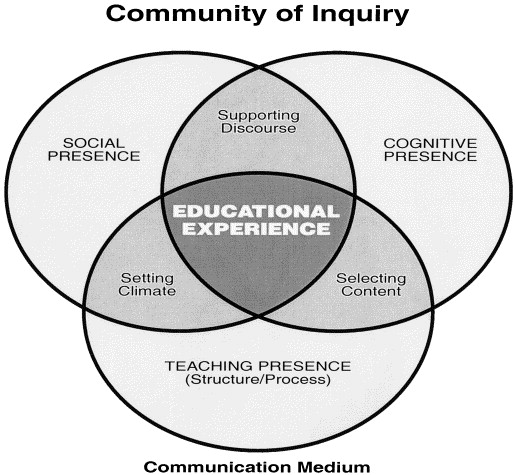
\includegraphics{assets/u1/CoI-Model.jpg}
\caption{Community of Inquiry Model}
\end{figure}

\hypertarget{cognitive-presence}{%
\subsubsection*{Cognitive Presence}\label{cognitive-presence}}
\addcontentsline{toc}{subsubsection}{Cognitive Presence}

Cognitive presence, possibly the most foundational element, is the
\textgreater{} extent to which the participants in any particular configuration of a community of inquiry are able to construct meaning through sustained communication (p.~89).

Recall that this cognitive process is at the heart of constructivist learning environments. It seems obvious (be careful when people say that) that this construction of meaning through communication is the entire point of higher education. Your task as a student is to change your own mind, and that is a very tall order as our beliefs about many things are remarkably resilient. The way we engage in this task will have a significant bearing on the outcomes of the task.

If we approach communication with too much confidence in our own views, we can shut out competing ideas to our own detriment, so it is important to bring a cautious intelligence, or, as I once heard a student describe it, epistemic humility. We all know that we are wrong about some things. The trouble is we don't know what we are wrong about and how we have misunderstood.

Cognitive presence in a text-based environment (like an online course) carries with it some affordances, but also some disadvantages. It is a relatively common experience for people to type something in a text message or an email, only to have their intentions grossly misunderstood because there are fewer para-linguistic cues in text compared to verbal face-to-face communication. Recent developments in incorporating emojis have started to change this, but emojis are generally considered to be too informal for `serious scholarly work' or written professional communication. So, the relatively lean environment of text can lead to significant misunderstandings.

On the other hand, for learners like me who tend toward introversion, the asynchronous nature of text-based learning environments is a huge advantage. I couldn't count the number of times that I have wanted to contribute to an in-class discussion, but needed too much time to formulate a coherent response, and before I knew it, the conversation had moved on. My point was no longer relevant, having been resolved by those in the class who were more extroverted and ready with an answer. A text-based environment, however, gives me \emph{time to think, write, revise, and then post} my response.

\hypertarget{social-presence}{%
\subsubsection*{Social Presence}\label{social-presence}}
\addcontentsline{toc}{subsubsection}{Social Presence}

Garrison, et.al. describe social presence as
\textgreater the ability of participants in the Community of Inquiry to project their personal characteristics into the community, thereby presenting themselves to the other participants as ``real people.'' (p.~89)

In any community, and especially the TWU community, the ability to \emph{belong} and to be accepted as a whole and integrated person is critical to people feeling like they \emph{actually do belong}. It is for this reason that many experienced online educators encourage a more colloquial style of writing in online forums or blogs. Strict adherence to APA or other style guides virtually eliminates self-referential language such as personal pronouns. It is hard to project your personal characteristics as a real person when you can only refer to yourself in the third person.

By allowing a more personal style and the projection of self into the community, it is thought that students will build a sense of trust in the community and feel more empowered to participate in the difficult work of changing their minds. Social presence supports cognitive presence by allowing the learning environment to be safe and welcoming.

\hypertarget{teaching-presence}{%
\subsubsection*{Teaching Presence}\label{teaching-presence}}
\addcontentsline{toc}{subsubsection}{Teaching Presence}

This final element of the CoI model is the design and facilitation of the learning experience
\textgreater to support and enhance social and cognitive presence for the purpose of realizing educational outcomes. (p.~90).

Teaching presence can be a shared function between members of the community. Garrison, et al.~point out that the design of the experience is typically performed by the teacher, and the facilitation is more often shared. In a connected course like this one, there is a greater emphasis on shared facilitation in a community of learners compared to what might be experienced in a f2f (face to face) course. It is in this shared discourse in a safe environment that allows learners to engage in the difficult cognitive work of learning.

\hypertarget{learning-activity}{%
\subsection*{Learning Activity}\label{learning-activity}}
\addcontentsline{toc}{subsection}{Learning Activity}

Read \href{https://www.sciencedirect.com/science/article/pii/S1096751600000166}{Critical inquiry in a text-based environment: Computer conferencing in higher education} (access through the TWU library).

If you haven't done so previously, sign up for and activate hypothes.is and while you are reading the article, leave some annotations that connect what you are reading to your own experience.

Use the tag `ldrs663' in any annotations you create so that we can all find each other.

\href{http://create.twu.ca/help/other-web-tools/hypothesis}{Click here for assistance getting set up with hypothes.is.}

As you read, consider a time where you experienced a learning environment where the three presences described in the CoI were apparent. Consider the following questions and consider writing your responses in a learning journal.
- Were all three presences demonstrated?
- Which of the three were most obvious? Least?
- Which presence is most important for you?

Note that this is an ungraded activity, but is designed to help prepare you for the assessments in this course. Throughout the course you are encouraged to take notes in a journal of some sort. Refer to these notes as you complete your assessments.

\hypertarget{topic-2-modes-of-interaction}{%
\section*{Topic 2: Modes of Interaction}\label{topic-2-modes-of-interaction}}
\addcontentsline{toc}{section}{Topic 2: Modes of Interaction}

For this next topic we will look at what we mean by `interaction', a word which is thrown around a lot in educational technology, but\ldots{}

\href{https://youtu.be/G2y8Sx4B2Sk}{Watch}

Before we get into the the topic of interaction, please take a few minutes to answer the following questions about scenarios that may or may not be considered `interaction'.
(Note that you can check your answer right away, and then click the arrow for the next example.)

{[}h5p id=``2''{]}

What do you think? Do you agree with the `correct' and `incorrect' responses on the quiz?

\hypertarget{interaction}{%
\subsection*{Interaction}\label{interaction}}
\addcontentsline{toc}{subsection}{Interaction}

Anderson (2003) argues that, despite the lack of clarity around definitions of interaction, there seems to be a general understanding that interaction of some sort is a requirement for learning. He settles on the definition from Wagner (1994, p.8)

\begin{quote}
reciprocal events that require at least two objects and two actions. Interactions occur when these objects and events mutually influence one another.
\end{quote}

He provides a model of interaction in learning environments that includes three main agents in the process: students, teachers, and content (Figure 1).

\begin{figure}
\centering
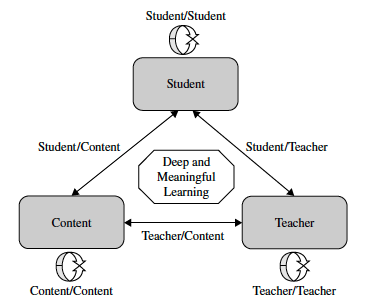
\includegraphics{assets/u1/Modes-Interaction-Anderson.png}
\caption{alt-text}
\end{figure}

Figure 1. Modes of Interaction from Anderson (2003).

At each point of the triangle are the agents in an educative process. The arrows between them indicate the two-way communication described by Wagner, and the recursive arrows above or below the agents are secondary forms of interaction.

\hypertarget{other-models-of-interaction}{%
\subsection*{Other Models of Interaction}\label{other-models-of-interaction}}
\addcontentsline{toc}{subsection}{Other Models of Interaction}

Kanuka (2011) describes a modified model of interaction which presumes that all educational interactions occur in the context of some sort of content (Figure 2.).

\begin{figure}
\centering
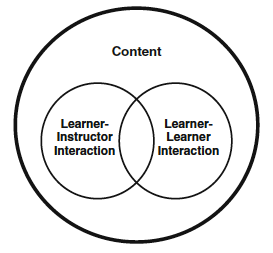
\includegraphics{assets/u1/Kanuka-Modes-of-Interaction.png}
\caption{alt-text}
\end{figure}

Figure 2. Modes of Interaction from Kanuka (2011).

In Anderson's model, content is an agent in the process, but in Kanuka's model, content of some sort is assumed to be the foundation of learning environments and that interactions between and among learners and instructors happens in the context of making sense of the content. The content itself does not have agency.

A combination of these two models was described by Madland (2014). Madland's model, shown in figure 3, is a return to Anderson's three-sided model except with the addition of peer interactions, and all interactions between agents occuring in the context of the content that is to be learned. Also added are the three sides of the model representing structured learning activities designed specifically to enhance the educative effects of the interactions.

\begin{figure}
\centering
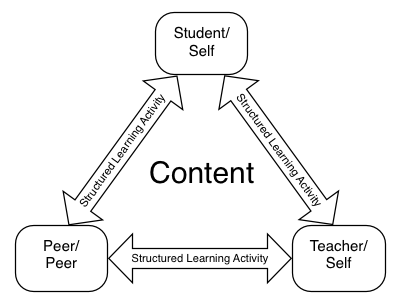
\includegraphics{assets/u1/Modes-of-Interaction-Madland.png}
\caption{alt-text}
\end{figure}

Figure 3. Modes of Interaction from Madland (2014).

\begin{quote}
Madland, C. (2014). \emph{Structured student interactions in online distance learning: Exploring the study buddy activity} (Master's thesis, Athabasca University). Retrieved from \url{http://hdl.handle.net/10791/47}
\end{quote}

It is not enough to simply expect interactions between learners and instructors to be goal-oriented towards learning outcomes. Educators must design specific activities (teaching presence) to create the conditions (social presence) for learning to occur (cognitive presence). An example of this can be seen in the seemingly ubiquitous `Group Project' assigned in so many undergraduate courses. Sometimes, groups are allowed to form themselves, other times, the instructor assigns groups, or there is some sort of random process to create groups. However they are formed, groups too often fall into a pattern of behaviour where one or two of the students do most of the work and the remaining group members engage in social loafing and benefit from their peers' work.

An alternative practice is to engage groups in a specific structured process of cooperation where everybody must do their work, or else the entire group suffers. An example is to have students work in peer review partners where students submit their assignments to their peer review partner who then provides feedback based on specific questions and categories of comments. When the original students receives their partner's feedback, they may choose how to integrate the suggestions into the final assignment that they submit to their instructor. Each student is then graded on the quality of their finished assignment, the quality of the feedback that they provided, and on the rationale for how they incorporated the peer review into their own work.

There are myriad structures that can be used to ensure that interactions are inclined towards producing student learning, and we will introduce you to some of those in unit 5.

\hypertarget{learning-activity-1}{%
\subsection*{Learning Activity}\label{learning-activity-1}}
\addcontentsline{toc}{subsection}{Learning Activity}

\hypertarget{read}{%
\subsubsection*{Read}\label{read}}
\addcontentsline{toc}{subsubsection}{Read}

Read the following article by Terry Anderson
- \href{http://www.irrodl.org/index.php/irrodl/article/view/149/230}{Getting the mix right again: An updated and theoretical rationale for interaction}

As you read, consider what interactions you have experiences in online or f2f courses.

\hypertarget{topic-3-interaction-equivalency-theorem}{%
\section*{Topic 3: Interaction Equivalency Theorem}\label{topic-3-interaction-equivalency-theorem}}
\addcontentsline{toc}{section}{Topic 3: Interaction Equivalency Theorem}

For our last topic of this unit, we'll explore Anderson's (2003) \emph{Interaction Equivalency Theorem}, stated as

\begin{quote}
Deep and meaningful formal learning is supported as long as one of the three forms of interaction (student--teacher; student-student; student-content) is at a high level. The other two may be offered at minimal levels, or even eliminated, without degrading the educational experience.
High levels of more than one of these three modes will likely provide a more satisfying educational experience, though these experiences may not be as cost or time effective as less interactive learning sequences. (p.~4)
\end{quote}

At TWU, there has always been a significant emphasis placed on student-teacher interactions. This can be seen in small class sizes and opportunities for students to be involved in faculty-led research projects and travel studies. Distance education, however, has long suffered from a distinct lack of student-teacher and student-student interactions. For many years, distance education was delivered either through the post or through one-way media such as radio or TV, virtually eliminating interactions. This led to a pervasive view that distance education courses and programs were second-rate at best.

However, now that modern communication infrastructure has developed to the point that media-rich, synchronous, two-way communication is almost free, opportunities for distance learning environments to include high levels of student-student and student-teacher interaction are much more feasible.

One problem remains, though, and that is that student-teacher interaction is a scarce commodity. It is costly to hire enough faculty to enable one-on-one or small-group interaction between students and faculty. The distance educator's response to this challenge is to front-load the faculty input (high-level disciplinary expertise or cognitive presence) into the course materials and to de-couple `interaction' from both time and place.

In an asynchronous, text-based environment, students and teachers do not need to be present in the same place at the same time in order to enjoy rich interactions.

\hypertarget{unit-1-assessment}{%
\section*{Unit 1 Assessment}\label{unit-1-assessment}}
\addcontentsline{toc}{section}{Unit 1 Assessment}

Please complete the assignment under `Post 1' below. This will be your first of five draft posts during the course.

\href{assessments/\#blog}{Blog Post 1}

\hypertarget{references}{%
\section*{References}\label{references}}
\addcontentsline{toc}{section}{References}

Anderson, T. (2003). Getting the mix right again: An updated and theoretical rationale for interaction. \emph{International Review of Research in Open and Distance Learning,} 4(2), 1--14.

Dewey, J. (1897). \emph{My pedagogic creed.} In M. S. Dworkin (Ed.), \emph{Dewey on education.} NewYork, NY: Teachers College Press.

Driscoll, M. P. (2005). \emph{Psychology of learning for instruction} (3rd ed.). Boston: Pearson Education.

Garrison, D. R., Anderson, T., \& Archer, W. (2000). Critical inquiry in a text-based environment: Computer conferencing in higher education. \emph{The Internet and Higher Education, 2}, 87--105. \url{https://doi.org/10.1016/S1096-7516(00)00016-6}

Kanuka, H. (2011). Interaction and the online distance classroom: Do instructional methods effect the quality of interaction? \emph{Journal of Computing in Higher Education,} 23(2), 143--156. \url{https://doi.org/10.1007/s12528-011-9049-4}

Madland, C. (2014). \emph{Structured student interactions in online distance learning: Exploring the study buddy activity} (Master's thesis). Athabasca University. Retrieved from \url{http://hdl.handle.net/10791/47}

\hypertarget{final-words}{%
\chapter{Final Words}\label{final-words}}

We have finished a nice book.

\hypertarget{methods-1}{%
\chapter{Methods}\label{methods-1}}

We describe our methods in this chapter.

Math can be added in body using usual syntax like this

\hypertarget{math-example-1}{%
\section{math example}\label{math-example-1}}

\(p\) is unknown but expected to be around 1/3. Standard error will be approximated

\[
SE = \sqrt(\frac{p(1-p)}{n}) \approx \sqrt{\frac{1/3 (1 - 1/3)} {300}} = 0.027
\]

You can also use math in footnotes like this\footnote{where we mention \(p = \frac{a}{b}\)}.

We will approximate standard error to 0.027\footnote{\(p\) is unknown but expected to be around 1/3. Standard error will be approximated

  \[
  SE = \sqrt(\frac{p(1-p)}{n}) \approx \sqrt{\frac{1/3 (1 - 1/3)} {300}} = 0.027
  \]}

\hypertarget{applications}{%
\chapter{Applications}\label{applications}}

Some \emph{significant} applications are demonstrated in this chapter.

\hypertarget{example-one}{%
\section{Example one}\label{example-one}}

\hypertarget{example-two}{%
\section{Example two}\label{example-two}}

\hypertarget{final-words-1}{%
\chapter{Final Words}\label{final-words-1}}

We have finished a nice book.

  \bibliography{book.bib}

\end{document}
